\ifdefined\ReaderVersion
  \documentclass[pdflatex,sn-vancouver-num,iicol]{sn-jnl}
\else
  \documentclass[pdflatex,sn-vancouver-num]{sn-jnl}
\fi

\usepackage{amsmath,amssymb,mathtools}
\usepackage{array,booktabs,multirow,tabularx}
\usepackage{graphicx,microtype}
\usepackage{url}
\ifdefined\ReaderVersion\else
  \usepackage[switch]{lineno}
  \usepackage{setspace}
\fi
\graphicspath{{figures/}}
\hypersetup{
  pdftitle={Fixed-margin prediction of cell-level RNA--surface-protein dependence across cohorts},
  pdfauthor={Anonymous Authors}
}
\input{manuscript_results_macros.tex}

\newcolumntype{Y}{>{\raggedright\arraybackslash}X}

\begin{document}
\raggedbottom
\ifdefined\ReaderVersion\else
  \newgeometry{left=25mm,right=25mm,top=23mm,bottom=25mm}
  \doublespacing
  \linenumbers
\fi

\title[Fixed-margin dependence prediction]{Fixed-margin prediction of cell-level RNA--surface-protein dependence across cohorts}

\author*[1]{\fnm{Anonymous} \sur{Authors}}
\affil*[1]{\orgdiv{Affiliations withheld in the blinded manuscript}}

\abstract{
\textbf{Background:} Linked single-cell assays resolve cross-modal dependence because they measure molecular states in the same cell. A recipient cohort may retain the marginal state counts of both assays without preserving cell-level pairing. Its joint table is then unobserved and cannot be recovered from the margins alone.

\textbf{Results:} We formulate fixed-margin prediction from paired source donors and unpaired recipient counts. Conditional models estimate source log odds; averaging over their transported distribution gives the table minimizing expected multinomial deviance under the transported model. In a prespecified CITE-seq study of nine RNA and nine protein markers, hierarchical transfer from 36 Cambridge donors reduced deviance by 17.46\% versus signed-statistic transfer across 56 Newcastle donors (paired-donor 95\% interval for the loss difference, $-0.00413$ to $-0.00080$). A matched post hoc comparison favored calibrated normal random-effects prediction. Its predictive mixture reduced deviance by 8.46\% relative to the original hierarchy (95\% interval, 5.42--11.55\%) and by 1.33\% relative to the same fit's population plug-in (0.72--1.96\%). With source-defined protein thresholds, hierarchical transfer retained a 2.70\% gain over common conditional estimation in 54 recipients (0.72--4.73\%). Cell-type-preserving permutations gave similar prediction loss. Ground-truth simulations separated the effects of margin shift, donor pooling, and predictive integration.

\textbf{Conclusions:} Linked source donors and recipient marginal counts support prediction of cross-modal joint tables. Conditioning separates marginal abundance from association; calibration and integration over donor variation improve the transported prediction.
}

\keywords{single-cell multi-omics; conditional likelihood; log-linear association; transfer learning; CITE-seq; reproducibility}

\maketitle

\section{Background}

Linked single-cell assays measure RNA, chromatin, proteins, molecular age, and lineage in the same cell or experimentally related unit \cite{papalexi2021,frangieh2021,totalvi2021,multivi2023,perturbsci2023,resistrace2024}. Joint latent-variable models integrate paired measurements or predict a missing modality. We consider a different information boundary: source donors have paired measurements, whereas a recipient provides only aggregate state counts for the same cell sample, with pairing withheld. The target is the recipient joint table that cell-level pairing would have revealed.

Marginal frequencies change with cell composition, activation, sequencing depth, and assay scale. Copying a source table therefore transfers abundance together with dependence. Signed Pearson and likelihood-ratio statistics summarize departure from independence, but their scale and attainable range depend on the margins. A statistic pooled across donors can consequently change meaning at recipient margins.

Log-linear interactions isolate association in contingency tables \cite{goodman1970,goodman1979,egozcue2015,facevicova2016}. Conditional likelihood removes row and column nuisance parameters; hierarchical conditional and random-effects log-linear models pool odds ratios across observed strata \cite{mantel1959,liao1999,coullagresti2003,stijnen2010}. Fixed-margin tables can be generated from specified log-linear dependence \cite{hammond2024}, and marginal distributions can be completed by odds-ratio coordinates in variation-independent parameterizations \cite{evansdidelez2024}. Categorical data fusion also studies joint distributions that are not directly observed, using proxies or other auxiliary identifying information \cite{zhang2015fusion}. Copula and differential-association methods estimate dependence from observed single-cell or multi-omic pairings \cite{ma2023,diffcoex2010,dgca2016,schot2020}.

We study prediction from paired source donors and unpaired recipient margins. Auxiliary-file statistical matching uses external joint observations to supply relationships missing from recipient data \cite{moretti2023}. Here, donor-stratified conditional estimation separates the source interaction from donor variation, and the recipient margins determine the feasible joint tables. The prediction minimizing expected multinomial deviance is their conditional mean. When recipient interactions vary, this mean averages over the predictive distribution of log odds. A pairing-blinded CITE-seq experiment and ground-truth simulations assess the roles of marginal reconstruction, donor pooling, and the prediction rule.

\begin{figure*}[t]
\centering
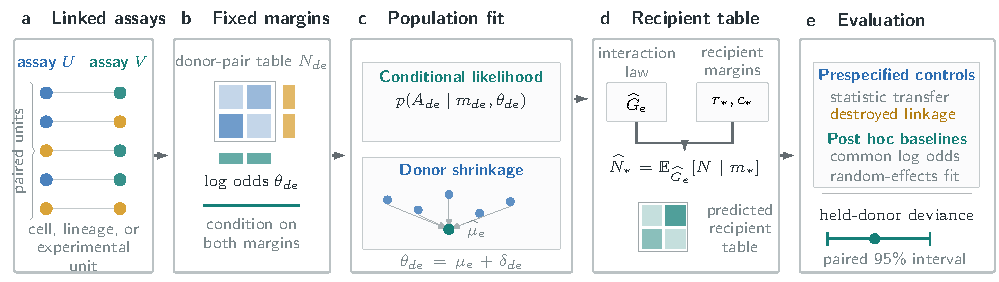
\includegraphics[width=\textwidth]{standalone_figures/figure1.pdf}
\caption{\textbf{Conditional prediction of pairwise dependence.} Linked source measurements define donor-level joint tables. Conditional estimation separates interaction from marginal abundance. The fitted interaction law and recipient margins determine the mean recipient table. A point-mass law gives population plug-in prediction; a distribution of interactions gives predictive integration. Comparisons retain the same source data and recipient margins.}
\label{fig:workflow}
\end{figure*}

\section{Methods}

\subsection{Association coordinates}

For ordered RNA--protein pair $e$, let $P_e$ be the positive joint-probability table of its binary states. Association is represented by the log odds ratio,
\begin{equation}
  \theta_e=\log\frac{P_{e,00}P_{e,11}}{P_{e,01}P_{e,10}}.
  \label{eq:logodds}
\end{equation}
Positive row and column tilts leave this interaction unchanged. Additional file 1 gives the multistate contrast representation and its invariance properties.

\subsection{Hierarchical conditional estimator}

For $D$ source donors, let $A_{de}$ be the upper-left count in the binary table for donor $d$ and marker pair $e$, and let $m_{de}$ denote its margins. Conditional on these margins, the table has one free count. Its exact distribution is
\begin{equation}
  p(a\mid m_{de},\theta)=
  \frac{w_{de}(a)\exp(\theta a)}
  {\sum_{b\in\mathcal A_{de}}w_{de}(b)\exp(\theta b)},
  \label{eq:conditionalmodel}
\end{equation}
where $\mathcal A_{de}$ is the feasible integer support and $w_{de}(a)$ is the central-hypergeometric combinatorial weight. The distribution depends on the log odds $\theta$ but not on row or column effects.

We write the donor-specific log odds as a population effect $\mu_e$ plus a donor deviation $\delta_{de}$. The estimator minimizes
\begin{equation}
\begin{aligned}
  \mathcal{L}(\mu,\delta)={}&-\frac{1}{D}\sum_{d,e}
  \log p(A_{de}\mid m_{de},\mu_e+\delta_{de})\\
  &+\frac{\gamma}{2}\sum_{d,e}\delta_{de}^{2}
  +\frac{\rho}{2}\lVert\mu\rVert_2^2.
  \label{eq:objective}
\end{aligned}
\end{equation}
The first term is the donor-normalized negative exact conditional log likelihood summed over marker pairs. The panel objective is composite because marker pairs from one donor reuse cells. The parameter $\gamma$ shrinks donor deviations toward the population interaction, and $\rho$ penalizes the population interaction. Penalty scaling, optimization, and convergence criteria are given in Additional file 1.

Conditioning a Poisson log-linear model on both margins removes every row and column parameter and yields Eq.~\eqref{eq:conditionalmodel}. Positive donor and population penalties give Eq.~\eqref{eq:objective} a unique finite minimizer; Proposition S2 in Additional file 1 gives the derivation and proof.

For recipient $q$, the prediction is the fixed-margin expected table at transported population log odds,
\begin{equation}
  \widehat N_{qe}=\mathbb{E}_{\alpha\widehat\mu_e}
  [N_{qe}\mid m_{qe}],
  \label{eq:prediction}
\end{equation}
where the development design selects $\alpha$ from a prespecified study grid. The binary cohort studies used $\{0.5,0.75,1,1.25\}$, and the longitudinal calibration also included zero. This table preserves the recipient margins without a pseudocount or post-fit projection.

Proposition S4 in Additional file 1 proves that the conditional mean in Eq.~\eqref{eq:prediction} uniquely minimizes expected multinomial deviance under the transported interaction. Proposition S3 separates source estimation error from recipient variation in the conditional log loss of a single transported log odds.

\subsection{Prediction with recipient variation}

A population log odds specifies one interaction, whereas a new donor can differ from the population. For a predictive distribution $G_e$ of recipient log odds, the corresponding mean table is
\begin{equation}
  \widehat N_{qe}^{\mathrm{mix}}
  =\int\mathbb E_{\theta}[N_{qe}\mid m_{qe}]\,dG_e(\theta).
  \label{eq:mixture-prediction}
\end{equation}
This prediction preserves both margins and minimizes expected recipient deviance under the mixture law. Evaluating the table at the mean log odds generally gives a different prediction because the conditional mean is nonlinear. The decision-regret result in Additional file 1 relates this difference directly to the evaluated table loss.

For a normal interaction distribution, we estimated the population mean and between-donor variance by exact conditional marginal maximum likelihood \cite{jackson2018}. The post hoc comparison evaluated both the population plug-in and mixture prediction from this fit. The original 12 calibration donors supplied each candidate fit, the 24 pilot donors selected its transport multiplier, and all 36 source donors supplied the final estimate. Multipliers scaled both the mean and standard deviation of log odds. Equal-tail 95\% intervals for the recipient upper-left count used the fitted predictive distribution.

\subsection{Classical comparisons and controls}

The matched statistic comparator transfers either the signed root Pearson statistic or the signed root likelihood-ratio deviance from the row-plus-column independence model. We normalized statistics by table size, pooled them across source donors, rescaled them for each recipient, and inverted them at its margins. The Stephenson protocol used Paule--Mandel random-effects pooling \cite{paule1982}. Each study fixed its pooling rule in advance; development data selected the statistic, any evaluated null centering, and the transport multiplier. Both methods received the same recipient margins without recipient pairings.

Two fitted interaction baselines compared alternative pooling rules. The common-effect conditional maximum-likelihood estimate fitted one unpenalized log odds per marker pair across donor strata. The pooled-table baseline used the sample log odds ratio of the donor-pooled table. In the post hoc comparison, both coefficients were reconstructed by fixed-margin conditional expectation with a development-selected transport multiplier. We report the second method as pooled-table log odds with conditional reconstruction.

The predictive reanalysis also fitted a common-effect conditional estimator with the same population ridge penalty, 0.01, as the hierarchy. The normal random-effects comparison used the same source tables, donor split, recipient margins, multiplier grid, and outcome. These analyses retained the original panel and donor weighting.

The destroyed-link control permuted complete protein profiles within each donor before joint tables were formed. This preserved RNA and protein margins and dependence within the protein panel but removed cell-level RNA-protein linkage. We refitted the selected conditional estimator to the permuted tables. Fixed-margin independence provided a further control.

For observed table $T$, positive prediction $\widehat T$, and table total $n$, the loss is multinomial deviance per cell,
\begin{equation}
  D(T,\widehat T)=\frac{2}{n}\sum_{i,j:T_{ij}>0}
  T_{ij}\log\frac{T_{ij}}{\widehat T_{ij}}.
  \label{eq:deviance}
\end{equation}
Entity losses were averaged within each evaluation unit. Confirmatory means weighted physical donors equally. The 95\% intervals used 20,000 paired bootstrap draws at the donor or prespecified batch-block level, conditional on the source fit, selected configuration, and deterministic cell sample. Development intervals resampled the displayed samples or batches.

\subsection{Ground-truth simulation}

We simulated \SimReps{} replicates from the exact fixed-margin model with known population log odds, 12 source donors, 12 recipient donors, 16 marker pairs, and 128 observations per table. Source donor effects were either homogeneous or normally heterogeneous with standard deviation 1.2; recipient log odds equaled the population value. Recipient margins either followed the source distribution or underwent a strong shift. Hyperparameters and transport multipliers were fixed across all four scenarios. Both conditional estimators used the same population ridge penalty of 0.01. Comparators also included raw and null-centered signed-root deviance-statistic transfer. Paired bootstrap intervals resampled simulation replicates in 20,000 draws.

An eight-scenario extension crossed source and recipient standard deviations of 0 or 1.2 with the same two margin conditions. It retained the original source draws and fitting settings. Predictions using known population parameters compared the population plug-in with the normal-mixture mean, separating decision-rule error from parameter-estimation error.

\subsection{Prespecified held evaluation}

The Stephenson analysis plan fixed eligibility, donor allocation, cell selection, state definitions, marker panels, tuning grids, comparators, loss, uncertainty, and success criteria before the Newcastle pairing outcomes were observed. The Cambridge pilot selected the final configuration from these grids, after which all Cambridge development donors supplied the final fit. Predictions used Newcastle margins alone and were recorded before RNA--protein pairing was restored for evaluation.

Confirmation required at least 5\% lower mean deviance than both the selected statistic-transfer and destroyed-link controls, a paired-bootstrap upper endpoint below zero, and a one-sided sign-test $P\leq0.025$. Model selection ended before the Newcastle pairing outcomes were observed.

\subsection{Datasets and state construction}

Stephenson et al. profiled PBMC RNA and surface proteins with a common TotalSeq-C panel across Cambridge and Newcastle \cite{stephenson2021}. The split used 12 Cambridge calibration donors, 24 Cambridge pilot donors, and 56 Newcastle donors for the held-site test. Nine cognate RNA and protein markers defined 81 ordered pairs.

Each donor contributed 512 cells selected by a deterministic rule that did not access RNA or ADT counts. RNA state recorded raw detection. Deterministic within-donor protein ranks assigned 256 low and 256 high cells, fixing every protein margin before evaluation.

\subsection{Biological sensitivities}

Two post hoc analyses retained the original donors, cells, marker panel, and hierarchical configuration. First, eight independent source permutations shuffled complete protein profiles within each donor and annotated cell type. This control preserved cell-type composition and within-type marginal distributions, removing RNA--protein pairing within the annotation strata. Intact and permuted source fits predicted the same original recipient tables.

Second, a fixed raw-count threshold for each protein was its pooled median across the 36 Cambridge donors. The same thresholds defined high protein states in Newcastle, allowing recipient protein prevalence to vary. Pair eligibility required informative margins in at least two source donors. The hierarchy and common conditional estimate used $\alpha=1$ without further tuning.

\section{Results}

\subsection{Association transferred across recruitment sites}

Across \StephHeldN{} Newcastle donors, the hierarchical conditional estimator reached mean deviance \StephPrimaryLoss{}, compared with \StephResidualLoss{} for signed-root deviance-statistic transfer. The corresponding \StephResidualReduction{} reduction had a paired-donor loss-difference interval of \StephResidualCILo{} to \StephResidualCIHi{}. The conditional estimate was better in \StephResidualFav{} donors ($P=\StephSignP$, one-sided sign test). All \StephDevN{} Cambridge development donors supplied the final source fit after pilot selection.

The estimator also reduced deviance by \StephDestroyedReduction{} relative to the destroyed-link fit of \StephDestroyedLoss{} (paired-donor interval \StephDestroyedCILo{} to \StephDestroyedCIHi{}; \StephDestroyedFav{} donors favorable). In post hoc fitted-baseline analyses, it improved on the common-effect conditional estimate by \StephCommonExactReduction{} (relative-reduction interval \StephCommonExactReductionLo{} to \StephCommonExactReductionHi{}) and on pooled-table log odds with conditional reconstruction by \StephPooledPoissonReduction{} (\StephPooledPoissonReductionLo{} to \StephPooledPoissonReductionHi{}).

\begin{table*}[t]
\caption{Held-site performance against matched controls and fitted interaction baselines.}
\label{tab:stephenson-results}
\centering
\small
\begin{tabularx}{\textwidth}{@{}Y Y r r Y r@{}}
\toprule
Comparator & Analysis role & Comparator loss & Reduction & Difference 95\% CI & Favorable donors \\
\midrule
Signed-root deviance transfer & prespecified & \StephResidualLoss & \StephResidualReduction & \StephResidualCILo{} to \StephResidualCIHi & \StephResidualFav \\
Destroyed source linkage & prespecified & \StephDestroyedLoss & \StephDestroyedReduction & \StephDestroyedCILo{} to \StephDestroyedCIHi & \StephDestroyedFav \\
Common-effect conditional estimate & fitted baseline & \StephCommonExactLoss & \StephCommonExactReduction & \StephCommonExactCILo{} to \StephCommonExactCIHi & \StephCommonExactFav \\
Pooled-table log odds & fitted baseline & \StephPooledPoissonLoss & \StephPooledPoissonReduction & \StephPooledPoissonCILo{} to \StephPooledPoissonCIHi & \StephPooledPoissonFav \\
\bottomrule
\multicolumn{6}{@{}p{.98\textwidth}@{}}{\footnotesize The hierarchical conditional loss was \StephPrimaryLoss{}. Differences are hierarchical minus comparator deviance per cell. Intervals use 20,000 paired donor-bootstrap draws. Fitted-baseline comparisons were specified after the held result and are descriptive.}\\
\end{tabularx}
\end{table*}

\subsection{Predictive integration improved calibrated transfer}

The post hoc comparison selected $\alpha=0.75$ for both normal random-effects predictions (Table~\ref{tab:predictive-comparison}). The mixture reached mean deviance 0.011165, an 8.46\% reduction relative to the original hierarchy (95\% interval, 5.42--11.55\%). It improved on common conditional estimation with matched ridge by 11.79\% (7.43--16.10\%). The population plug-in from the same random-effects fit reached 0.011315. Integrating its fitted variation reduced deviance by 1.33\% (0.72--1.96\%; 38/56 donors favorable), isolating the effect of the prediction rule.

Calibration also mattered. Without rescaling log odds, random-effects plug-in and mixture losses were 0.013865 and 0.013137, both above the original hierarchy. The calibrated mixture reduced loss by 24.44\% relative to the frozen statistic comparator (95\% interval, 16.03--31.16\%). Equal-tail 95\% count-interval coverage was 70.01\% for the calibrated plug-in and 83.17\% for the mixture; mean interval widths were 15.74 and 22.90 cells.

\begin{table*}[t]
\caption{Post hoc prediction comparison under the original donor split. Lower deviance is better.}
\label{tab:predictive-comparison}
\centering\small
\begin{tabularx}{\textwidth}{@{}Y r r r r@{}}
\toprule
Estimator & $\alpha$ & 56-donor deviance & 54-donor sensitivity & 56-donor coverage \\
\midrule
Original hierarchy & 1 & 0.012197 & 0.011393 & --- \\
Common conditional, matched ridge & 1 & 0.012657 & 0.011713 & --- \\
Normal random effects, plug-in & 0.75 & 0.011315 & 0.010723 & 70.01\% \\
Normal random effects, mixture & 0.75 & 0.011165 & 0.010622 & 83.17\% \\
\bottomrule
\multicolumn{5}{@{}p{.98\textwidth}@{}}{\footnotesize The pilot selected each multiplier before recipient scoring. The sensitivity excludes two low-signal protein panels without changing fits or predictions. Coverage is the donor-equal fraction of informative upper-left counts within nominal 95\% predictive intervals; parameter uncertainty is not included. Additional file 1 reports interval widths, uncertainty, and unscaled predictions.}\\
\end{tabularx}
\end{table*}

\subsection{Composition and protein-state controls}

Two original held donors had only 0 and 3 counts across the selected nine-protein panel; the next-lowest total across the other 90 source and recipient donors was 6,560. A post hoc sensitivity retained the published predictions for the other 54 recipients. Their mean hierarchical deviance was 0.011393, a 23.69\% reduction relative to statistic transfer (95\% interval, 17.86--28.99\%; 50/54 donors favorable) and a 4.77\% reduction relative to common conditional estimation (2.99--6.53\%; 44/54 favorable). The original 56-donor result was unchanged.

In these 54 recipients, the calibrated mixture retained a 6.77\% gain over the original hierarchy (95\% interval, 4.41--9.26\%) and a 0.95\% gain over its matched plug-in (0.55--1.36\%; 36/54 donors favorable). Its mean deviance was 0.010622.

With source-defined protein thresholds, 54 recipient donors had informative pairs. The hierarchy reached mean deviance 0.007927, compared with 0.008147 for common conditional estimation: a 2.70\% reduction (paired-donor 95\% interval, 0.72--4.73\%; 31/54 donors favorable). The same two low-signal donors had no informative pairs under this state definition.

All eight composition-preserving source fits converged. Their mean recipient deviance was 0.011867, compared with 0.012197 for intact source linkage. The intact-minus-control difference was 0.000330 (paired-donor 95\% interval, $-0.000335$ to 0.001096; 31/56 donors favorable to intact linkage). Nested resampling over donors and source permutations gave a similar interval, $-0.000336$ to 0.001087.

\subsection{Conditioning and donor shrinkage separated distinct errors}

The factorial simulation separated donor heterogeneity from margin shift (Fig.~\ref{fig:simulation}). With heterogeneous donor effects and source-like margins, the hierarchical estimator reached deviance \SimHetSameHier{}, compared with \SimHetSameCommon{} for the common-effect conditional estimate. The reduction was \SimHetSameCommonReduction{} (95\% interval \SimHetSameCommonReductionLo{} to \SimHetSameCommonReductionHi{}). After the recipient margins shifted, conditional transport reduced deviance by \SimHetShiftResidualReduction{} (\SimHetShiftResidualReductionLo{} to \SimHetShiftResidualReductionHi{}) relative to raw signed-root deviance-statistic transfer.

Under homogeneous donor effects and source-like margins, common-effect conditional deviance was \SimHomSameCommon{}, compared with \SimHomSameHier{} for the hierarchical estimator, a shrinkage cost of \SimHomSameHierPenalty{}. After margin shift, the two conditional estimators remained close (\SimHomShiftCommon{} and \SimHomShiftHier{}), whereas statistic-transfer deviance rose to \SimHomShiftResidual{}. Fixed-margin reconstruction therefore absorbed the marginal shift in this model; donor shrinkage contributed when source associations varied across donors.

When both source and recipient log odds varied with standard deviation 1.2, the hierarchical reduction relative to matched-ridge common estimation was 0.41\% (95\% interval, 0.33--0.49\%) with source-like margins and 0.39\% (0.31--0.47\%) after margin shift. With population parameters known, integrating recipient variation reduced deviance relative to the population plug-in by 0.32\% (0.22--0.42\%) and 2.25\% (1.88--2.61\%), respectively. The latter comparison isolates the prediction rule from estimation of the interaction distribution. Additional file 1 reports all eight scenarios.

\begin{figure*}[t]
\centering
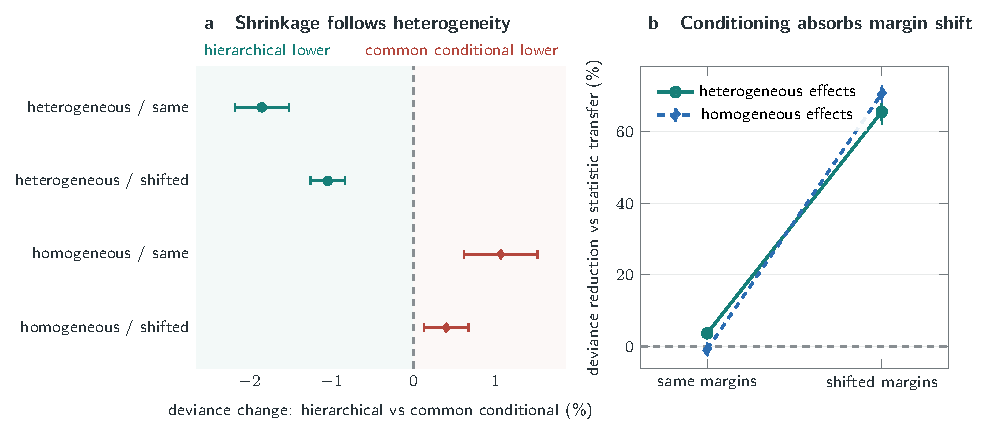
\includegraphics[width=\textwidth]{standalone_figures/figure2.pdf}
\caption{\textbf{Ground-truth estimator behavior.} \textbf{a}, relative change in recipient deviance for the hierarchical estimator against the common-effect conditional estimate. Negative values favor hierarchical shrinkage. \textbf{b}, reduction in deviance relative to raw signed-root deviance-statistic transfer before and after recipient-margin shift. Recipient log odds equal the population value in these four scenarios. Bars are 95\% paired simulation-replicate bootstrap intervals across \SimReps{} replicates.}
\label{fig:simulation}
\end{figure*}

\section{Discussion}

Recipient margins and donor variation govern different parts of the prediction. Fixed-margin reconstruction absorbed abundance shifts in simulation and transferred RNA--surface-protein dependence from Cambridge to Newcastle without copying source marginal frequencies. The original hierarchy improved on common conditional estimation, but the matched comparison favored calibrated normal random effects. Integrating the fitted interaction distribution further improved prediction over its population plug-in, consistent with the decision rule derived for recipient deviance. The gain persisted after excluding the two low-signal protein panels.

Classical stratified odds-ratio models estimate association among observed tables; fixed-margin construction combines known margins with specified dependence. We join these operations in a predictive study design whose recipient pairing is absent at fit time. The statistic-transfer and conditional estimators receive the same linked source tables and recipient margins. Models such as totalVI and MultiVI solve missing-modality problems from paired observations or cell-level covariates; fitting them to recipient cells would change this information boundary. Exact conditional random-effects estimation supplies the direct classical comparison for transporting donor-varying log odds.

\section{Limitations}

The held confirmation is observational and does not establish perturbation causality, molecular binding, or a regulatory mechanism. It uses binary states, 512 cells per donor, and nine RNA and nine protein markers. Shuffling within annotated cell types retained prediction accuracy, so the held-site result does not isolate within-cell-type dependence from association induced by cell composition. Source-defined protein thresholds extended the analysis beyond fixed 256/256 protein margins, but they are not validated positivity thresholds. Other cell budgets, broader panels, technologies, tissues, and state resolutions require independent replication. The 81 pairwise tables within a donor reuse cells and marker vectors; they do not specify a full multivariate cell distribution.

The held-site selection assigned no weight to graph regularization, so the empirical claim concerns hierarchical conditional transfer without graph or hypergraph smoothing. The fitted-interaction comparisons, predictive reanalysis, and biological sensitivities followed the held result and are not independent confirmations. Two recipients had almost no counts across the selected protein panel; median ranking nevertheless assigned balanced states through tie breaking. Their exclusion is a post hoc sensitivity, not a revision of the original confirmation.

Predictive integration assumes that the source interaction distribution applies to the recipient after calibration. Neither interval family achieved nominal 95\% coverage. The count intervals condition on fitted parameters and do not include source-parameter uncertainty. Donor bootstrap intervals likewise condition on the fitted model, selected configuration, and cell subsamples. Normal random-effects estimation and predictive averaging are established statistical procedures; the results support their use in this prediction setting, not superiority of a new likelihood family.

The Stephenson sign test is study specific and does not correct familywise error across the preceding search of public datasets. Its confirmatory interpretation applies to the prespecified experiment, not to the full development program. Of six binary studies, one reached a pre-outcome held-site test, one was corrected after outcome access, two stopped at calibration or pilot evaluation, and two stopped at source or eligibility checks. Additional file 1 retains their outcomes. The public ledger contains 37 analyses, including reused cohorts and later investigations, not 37 independent studies or preceding significance tests.

Conditioning on random margins can discard finite-sample information about an odds ratio under multinomial or independent-binomial sampling. The lost fraction converges to zero under standard large-sample conditions \cite{schervish2025}, but we did not quantify that loss for these sparse marker tables. Our recipient information boundary makes the margins observed constraints; it does not imply that conditioning is universally more efficient than an unconditional model when full recipient tables are available.

The exploratory multistate extension depends on discretization, a pseudocount, and finite permutation centering. Spatial applications require linked source observations at a defined sampling unit; unpaired source regional summaries do not identify the interaction to be transported.

\section{Conclusions}

Fixed-margin prediction reconstructs cell-level cross-modal dependence from linked source donors and recipient aggregate counts. The prespecified held-site experiment supported conditional transfer over matched statistic transfer and destroyed source linkage. A subsequent matched comparison improved prediction through calibrated normal random effects and integration over donor variation. Recipient margins, interaction calibration, and predictive averaging address distinct parts of the transfer problem.

\section*{Abbreviations}
ADT: antibody-derived tag; PBMC: peripheral blood mononuclear cell; RNA: ribonucleic acid.

\section*{Declarations}

\subsection*{Ethics approval and consent to participate}
This study used only public, de-identified data and involved no new participants, specimens, interventions, or identifiable records; the original studies report their ethics approvals and consent procedures.

\subsection*{Consent for publication}
Not applicable.

\subsection*{Availability of data and materials}
All source datasets are public through the accessions listed in Additional file 1 and retain their original licenses. Analysis plans, MIT-licensed software, cohort and simulation results, and study records are available in the \href{https://github.com/sushaan-k/coupling-fields-benchmark/releases/tag/coupling-fields-v2.0.4-public-benchmark}{v2.0.4 public release}. Raw matrices are not redistributed.

\subsection*{Competing interests}
Competing-interest information is withheld in the blinded manuscript.

\subsection*{Funding}
Funding information is withheld in the blinded manuscript.

\subsection*{Authors' contributions}
Author names and contribution statements are withheld in the blinded manuscript.

\subsection*{Acknowledgements}
OpenAI Codex assisted with code development, literature retrieval, manuscript editing, and \LaTeX{} preparation.

\subsection*{Additional file}
Additional file 1 (PDF). \emph{Mathematical results and public benchmark details}. Proofs, algorithms, dataset provenance, study status, comparator definitions, sensitivity analyses, and reproducibility information.

\bibliography{references}

\end{document}
